\documentclass[]{article}
\usepackage{lmodern}
\usepackage{amssymb,amsmath}
\usepackage{ifxetex,ifluatex}
\usepackage{fixltx2e} % provides \textsubscript
\ifnum 0\ifxetex 1\fi\ifluatex 1\fi=0 % if pdftex
  \usepackage[T1]{fontenc}
  \usepackage[utf8]{inputenc}
\else % if luatex or xelatex
  \ifxetex
    \usepackage{mathspec}
    \usepackage{xltxtra,xunicode}
  \else
    \usepackage{fontspec}
  \fi
  \defaultfontfeatures{Mapping=tex-text,Scale=MatchLowercase}
  \newcommand{\euro}{€}
\fi
% use upquote if available, for straight quotes in verbatim environments
\IfFileExists{upquote.sty}{\usepackage{upquote}}{}
% use microtype if available
\IfFileExists{microtype.sty}{%
\usepackage{microtype}
\UseMicrotypeSet[protrusion]{basicmath} % disable protrusion for tt fonts
}{}
\usepackage[margin=1in]{geometry}
\usepackage{color}
\usepackage{fancyvrb}
\newcommand{\VerbBar}{|}
\newcommand{\VERB}{\Verb[commandchars=\\\{\}]}
\DefineVerbatimEnvironment{Highlighting}{Verbatim}{commandchars=\\\{\}}
% Add ',fontsize=\small' for more characters per line
\usepackage{framed}
\definecolor{shadecolor}{RGB}{248,248,248}
\newenvironment{Shaded}{\begin{snugshade}}{\end{snugshade}}
\newcommand{\KeywordTok}[1]{\textcolor[rgb]{0.13,0.29,0.53}{\textbf{{#1}}}}
\newcommand{\DataTypeTok}[1]{\textcolor[rgb]{0.13,0.29,0.53}{{#1}}}
\newcommand{\DecValTok}[1]{\textcolor[rgb]{0.00,0.00,0.81}{{#1}}}
\newcommand{\BaseNTok}[1]{\textcolor[rgb]{0.00,0.00,0.81}{{#1}}}
\newcommand{\FloatTok}[1]{\textcolor[rgb]{0.00,0.00,0.81}{{#1}}}
\newcommand{\CharTok}[1]{\textcolor[rgb]{0.31,0.60,0.02}{{#1}}}
\newcommand{\StringTok}[1]{\textcolor[rgb]{0.31,0.60,0.02}{{#1}}}
\newcommand{\CommentTok}[1]{\textcolor[rgb]{0.56,0.35,0.01}{\textit{{#1}}}}
\newcommand{\OtherTok}[1]{\textcolor[rgb]{0.56,0.35,0.01}{{#1}}}
\newcommand{\AlertTok}[1]{\textcolor[rgb]{0.94,0.16,0.16}{{#1}}}
\newcommand{\FunctionTok}[1]{\textcolor[rgb]{0.00,0.00,0.00}{{#1}}}
\newcommand{\RegionMarkerTok}[1]{{#1}}
\newcommand{\ErrorTok}[1]{\textbf{{#1}}}
\newcommand{\NormalTok}[1]{{#1}}
\usepackage{graphicx}
\makeatletter
\def\maxwidth{\ifdim\Gin@nat@width>\linewidth\linewidth\else\Gin@nat@width\fi}
\def\maxheight{\ifdim\Gin@nat@height>\textheight\textheight\else\Gin@nat@height\fi}
\makeatother
% Scale images if necessary, so that they will not overflow the page
% margins by default, and it is still possible to overwrite the defaults
% using explicit options in \includegraphics[width, height, ...]{}
\setkeys{Gin}{width=\maxwidth,height=\maxheight,keepaspectratio}
\ifxetex
  \usepackage[setpagesize=false, % page size defined by xetex
              unicode=false, % unicode breaks when used with xetex
              xetex]{hyperref}
\else
  \usepackage[unicode=true]{hyperref}
\fi
\hypersetup{breaklinks=true,
            bookmarks=true,
            pdfauthor={JcB},
            pdftitle={DP},
            colorlinks=true,
            citecolor=blue,
            urlcolor=blue,
            linkcolor=magenta,
            pdfborder={0 0 0}}
\urlstyle{same}  % don't use monospace font for urls
\setlength{\parindent}{0pt}
\setlength{\parskip}{6pt plus 2pt minus 1pt}
\setlength{\emergencystretch}{3em}  % prevent overfull lines
\setcounter{secnumdepth}{5}

%%% Use protect on footnotes to avoid problems with footnotes in titles
\let\rmarkdownfootnote\footnote%
\def\footnote{\protect\rmarkdownfootnote}

%%% Change title format to be more compact
\usepackage{titling}
\setlength{\droptitle}{-2em}
  \title{DP}
  \pretitle{\vspace{\droptitle}\centering\huge}
  \posttitle{\par}
  \author{JcB}
  \preauthor{\centering\large\emph}
  \postauthor{\par}
  \predate{\centering\large\emph}
  \postdate{\par}
  \date{01/10/2014}




\begin{document}

\maketitle


{
\hypersetup{linkcolor=black}
\setcounter{tocdepth}{2}
\tableofcontents
}
\section{Analyse des diagnostics
principaux}\label{analyse-des-diagnostics-principaux}

Pour l'analyse, le fichier doit s'appeler dx. Ainsi pour 2014 on mettra
dans le préambule dx \textless{}- d14.

\begin{verbatim}
## Loading required package: foreign
## Loading required package: survival
## Loading required package: MASS
## Loading required package: nnet
## 
## Attaching package: 'epitools'
## 
## The following object is masked from 'package:survival':
## 
##     ratetable
## 
## Loading required package: zoo
## 
## Attaching package: 'zoo'
## 
## The following objects are masked from 'package:base':
## 
##     as.Date, as.Date.numeric
\end{verbatim}

\section{Combien de sorte de DP sont crées par jour
?}\label{combien-de-sorte-de-dp-sont-crees-par-jour}

ex. avec Sélestat: on crée un objet de type liste formé d'autant de
listes qu'il y a de jours (1 liste par jour). Chaque liste est formée
par les codes CIM10 du jour, lesquels ont regroupés par type grace à la
méthode table. Au final on obtient pour chaque jour la liste des codes
CIM et pour chaque code, le nombre de dossiiers correspondants. Par la
fonction \emph{length} on compte le nombre de diagnostics uniques.
L'ensemble est résumé par la fonction \emph{summary}.

\begin{verbatim}
[1] 65
\end{verbatim}

\begin{verbatim}

 B432  C719  D649  H650  H660  H813  I269  J040  J159  J181  J188  J209 
    1     1     1     1     1     1     1     1     1     2     1     2 
 J302  J451  J961  K528  K580  K590  K625  L022  L024  L028  L500  M139 
    1     1     1     1     1     1     1     1     1     1     1     1 
 M544 M5459  N188   N23  N300  N390  R040  R074  R100   R33  R509   R51 
    1     1     1     1     1     2     1     4     1     1     1     1 
R53+1  R600  S011  S015  S018 S0600  S223  S300 S3200 S4220  S430  S460 
    1     1     1     1     3     2     1     1     1     1     1     1 
 S520 S5250  S602  S610  S611 S6260 S6261  S800  S801 S8240  S901  S934 
    1     1     1     2     1     1     1     2     1     1     2     6 
 S936  T173  T435  Z020  Z711 
    1     1     1     1     1 
\end{verbatim}

\begin{verbatim}
   Min. 1st Qu.  Median    Mean 3rd Qu.    Max. 
    0.0    57.0    63.0    61.5    69.0    88.0 
\end{verbatim}

\begin{figure}[htbp]
\centering
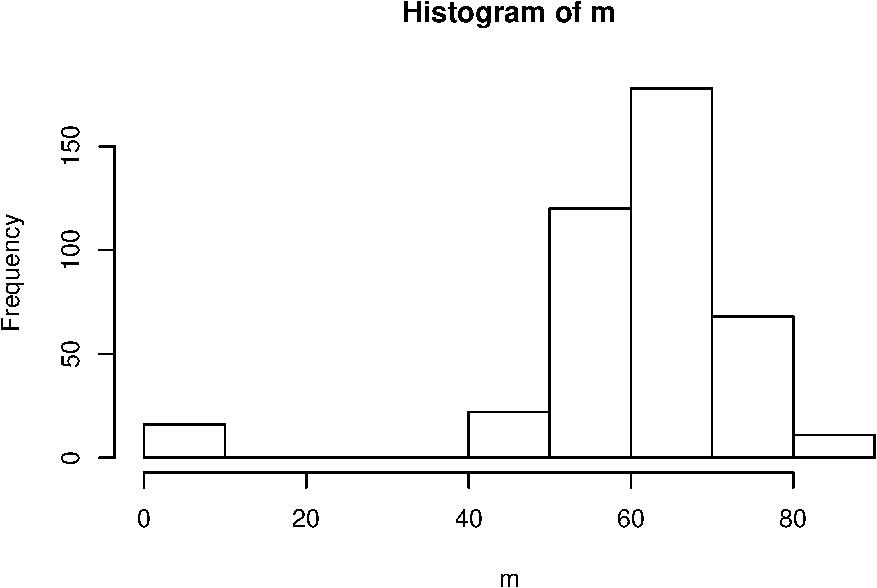
\includegraphics{dp_files/figure-latex/diag_par_jour-1.pdf}
\end{figure}

\section{Bronchiolites}\label{bronchiolites}

\begin{Shaded}
\begin{Highlighting}[]
\NormalTok{bron<-dpr[}\KeywordTok{substr}\NormalTok{(dpr$DP,}\DecValTok{1}\NormalTok{,}\DecValTok{3}\NormalTok{)==}\StringTok{"J21"} \NormalTok{&}\StringTok{ }\NormalTok{dpr$AGE <}\StringTok{ }\DecValTok{10} \NormalTok{,] }\CommentTok{# on limite aux moins de 10 ans}
\NormalTok{n.bron <-}\StringTok{ }\KeywordTok{nrow}\NormalTok{(bron) }\CommentTok{# nombre de bronchiolites}
\CommentTok{# age des bronchioloites en mois}
\NormalTok{age.bron <-}\StringTok{ }\NormalTok{(}\KeywordTok{as.Date}\NormalTok{(bron$ENTREE) -}\StringTok{ }\KeywordTok{as.Date}\NormalTok{(bron$NAISSANCE))/}\DecValTok{30}

\NormalTok{n2 <-}\StringTok{ }\KeywordTok{length}\NormalTok{(age.bron[age.bron <}\StringTok{ }\DecValTok{25}\NormalTok{]) }\CommentTok{# nb de 24 mois (2 ans)}
\KeywordTok{round}\NormalTok{(n2 *}\StringTok{ }\DecValTok{100} \NormalTok{/}\StringTok{ }\NormalTok{n.bron, }\DecValTok{2}\NormalTok{) }\CommentTok{# % de 2 ans et moins}
\end{Highlighting}
\end{Shaded}

\begin{verbatim}
## [1] 96.79
\end{verbatim}

\begin{Shaded}
\begin{Highlighting}[]
\NormalTok{titre <-}\StringTok{ }\KeywordTok{paste0}\NormalTok{(}\StringTok{"Bronchiolites"}\NormalTok{, }\StringTok{" - "}\NormalTok{, anc)}

\NormalTok{m<-}\KeywordTok{month}\NormalTok{(bron$ENTREE,}\DataTypeTok{label=}\NormalTok{T)}
\KeywordTok{barplot}\NormalTok{(}\KeywordTok{table}\NormalTok{(m),}\DataTypeTok{main =} \NormalTok{titre, }\DataTypeTok{xlab=}\StringTok{"Mois"}\NormalTok{, }\DataTypeTok{ylab =} \StringTok{"nombre de RPU"}\NormalTok{)}
\end{Highlighting}
\end{Shaded}

\begin{figure}[htbp]
\centering
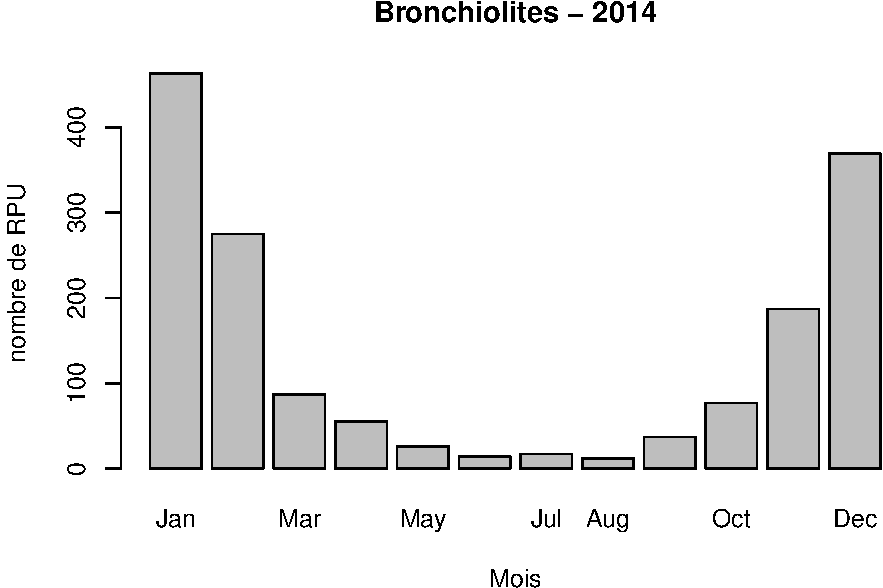
\includegraphics{dp_files/figure-latex/bronchiolites-1.pdf}
\end{figure}

\begin{Shaded}
\begin{Highlighting}[]
\CommentTok{# nombre de bronchiolites par semaine}
\NormalTok{s<-}\KeywordTok{week}\NormalTok{(bron$ENTREE)}
\NormalTok{n.bronchio.par.semaine <-}\StringTok{ }\KeywordTok{table}\NormalTok{(s)}
\KeywordTok{barplot}\NormalTok{(}\KeywordTok{table}\NormalTok{(s),}\DataTypeTok{main =} \NormalTok{titre, }\DataTypeTok{xlab =} \StringTok{"Semaines"}\NormalTok{, }\DataTypeTok{ylab =} \StringTok{"nombre de RPU"}\NormalTok{, }\DataTypeTok{las =} \DecValTok{2}\NormalTok{, }\DataTypeTok{cex.names =} \FloatTok{0.8}\NormalTok{)}
\end{Highlighting}
\end{Shaded}

\begin{figure}[htbp]
\centering
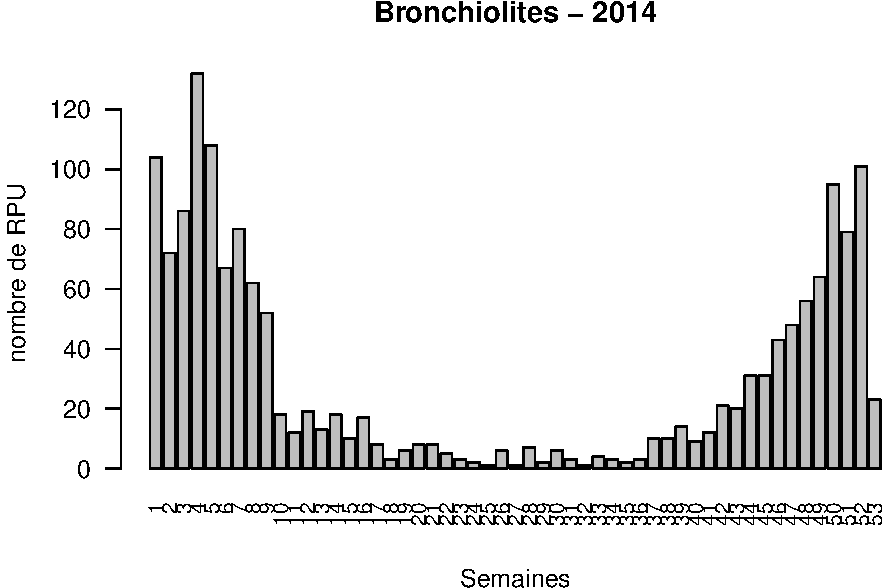
\includegraphics{dp_files/figure-latex/bronchiolites-2.pdf}
\end{figure}

\begin{Shaded}
\begin{Highlighting}[]
\CommentTok{# ages des enfants en mois}
\NormalTok{age.bron <-}\StringTok{ }\NormalTok{(}\KeywordTok{as.Date}\NormalTok{(bron$ENTREE) -}\StringTok{ }\KeywordTok{as.Date}\NormalTok{(bron$NAISSANCE))/}\DecValTok{30}
\NormalTok{s.age.bron <-}\StringTok{ }\KeywordTok{summary}\NormalTok{(}\KeywordTok{as.numeric}\NormalTok{(age.bron)) }\CommentTok{# résumé}
\KeywordTok{ceiling}\NormalTok{(}\KeywordTok{as.numeric}\NormalTok{(s.age.bron[}\StringTok{"Min."}\NormalTok{] *}\StringTok{ }\DecValTok{30}\NormalTok{)) }\CommentTok{# age min en jours}
\end{Highlighting}
\end{Shaded}

\begin{verbatim}
## [1] 7
\end{verbatim}

\begin{Shaded}
\begin{Highlighting}[]
\CommentTok{# sexe}
\KeywordTok{summary}\NormalTok{(bron$SEXE)}
\end{Highlighting}
\end{Shaded}

\begin{verbatim}
##    F    M         I 
##  606 1012    0    1
\end{verbatim}

\begin{Shaded}
\begin{Highlighting}[]
\CommentTok{# age de tous les RPU en jours}
\NormalTok{age.jours <-}\StringTok{ }\KeywordTok{as.numeric}\NormalTok{(}\KeywordTok{as.Date}\NormalTok{(dx$ENTREE) -}\StringTok{ }\KeywordTok{as.Date}\NormalTok{(dx$NAISSANCE))}

\CommentTok{# age de tous les rpu en mois}
\NormalTok{age.en.mois <-}\StringTok{ }\KeywordTok{as.numeric}\NormalTok{(}\KeywordTok{as.Date}\NormalTok{(dx$ENTREE) -}\StringTok{ }\KeywordTok{as.Date}\NormalTok{(dx$NAISSANCE))/}\DecValTok{30}

\CommentTok{# nb de rpu de moins de 24 mois}
\NormalTok{ped2.age <-}\StringTok{ }\NormalTok{age.en.mois[age.en.mois >}\StringTok{ }\DecValTok{0} \NormalTok{&}\StringTok{ }\NormalTok{age.en.mois <}\StringTok{ }\FloatTok{24.1}\NormalTok{]}
\KeywordTok{summary}\NormalTok{(ped2.age)}
\end{Highlighting}
\end{Shaded}

\begin{verbatim}
##     Min.  1st Qu.   Median     Mean  3rd Qu.     Max. 
##  0.03333  4.53300 10.63000 10.87000 16.77000 24.07000
\end{verbatim}

\begin{Shaded}
\begin{Highlighting}[]
\CommentTok{# il faut calculer le nombre de rpu de moins de 2 ans par semaine, puis voir ce que les bronchiolites représentent en %}

\NormalTok{a <-}\StringTok{ }\KeywordTok{data.frame}\NormalTok{(dx$ENTREE, age.en.mois)}
\NormalTok{a <-}\StringTok{ }\NormalTok{a[a$age.en.mois >}\StringTok{ }\DecValTok{0} \NormalTok{&}\StringTok{ }\NormalTok{a$age.en.mois <}\StringTok{ }\FloatTok{24.1}\NormalTok{,]}
\KeywordTok{colnames}\NormalTok{(a) <-}\StringTok{ }\KeywordTok{c}\NormalTok{(}\StringTok{"ENTREE"}\NormalTok{, }\StringTok{"AGE.MOIS"}\NormalTok{)}


\CommentTok{# nombre de passages des moins de 2 ans par semaine}
\CommentTok{# NB: semaine 41 = nouveau flux des HUS}
\NormalTok{n.rpu.inf2ans.par.semaine <-}\StringTok{ }\KeywordTok{tapply}\NormalTok{(}\KeywordTok{as.Date}\NormalTok{(a$ENTREE), }\KeywordTok{week}\NormalTok{(}\KeywordTok{as.Date}\NormalTok{(a$ENTREE)), length)}
\KeywordTok{barplot}\NormalTok{(n.rpu.inf2ans.par.semaine, }\DataTypeTok{main =} \StringTok{"Passages des moins de 2 ans"}\NormalTok{, }\DataTypeTok{ylab =} \StringTok{"nombre de RPU"}\NormalTok{, }\DataTypeTok{xlab =} \StringTok{"semaines"}\NormalTok{)}
\end{Highlighting}
\end{Shaded}

\begin{figure}[htbp]
\centering
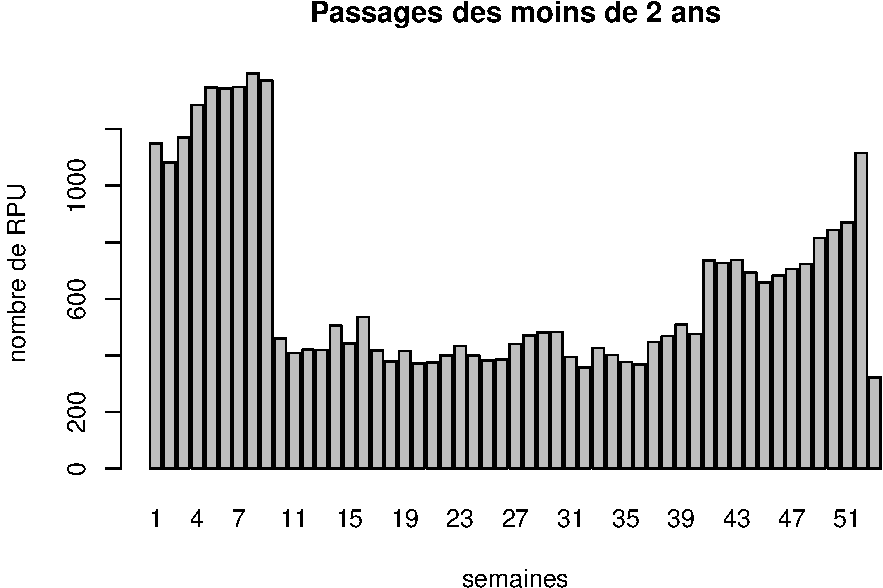
\includegraphics{dp_files/figure-latex/bronchiolites-3.pdf}
\end{figure}

\begin{Shaded}
\begin{Highlighting}[]
\CommentTok{# Pourcentage de bronchiolites par rapport au nombre total de passages d'enfants de moins de 24 mois}
\NormalTok{a <-}\StringTok{ }\KeywordTok{round}\NormalTok{(n.bronchio.par.semaine *}\StringTok{ }\DecValTok{100} \NormalTok{/}\StringTok{ }\NormalTok{n.rpu.inf2ans.par.semaine, }\DecValTok{2}\NormalTok{)}
\KeywordTok{barplot}\NormalTok{(a, }\DataTypeTok{xlab =} \StringTok{"semaines"}\NormalTok{, }\DataTypeTok{ylab =} \StringTok{"% de bronchiolites"}\NormalTok{, }\DataTypeTok{main =} \StringTok{"Pourcentage de bronchiolites par rapport au nombre total de passages}\CharTok{\textbackslash{}n}\StringTok{ d'enfants de moins de 24 mois"}\NormalTok{)}
\end{Highlighting}
\end{Shaded}

\begin{figure}[htbp]
\centering
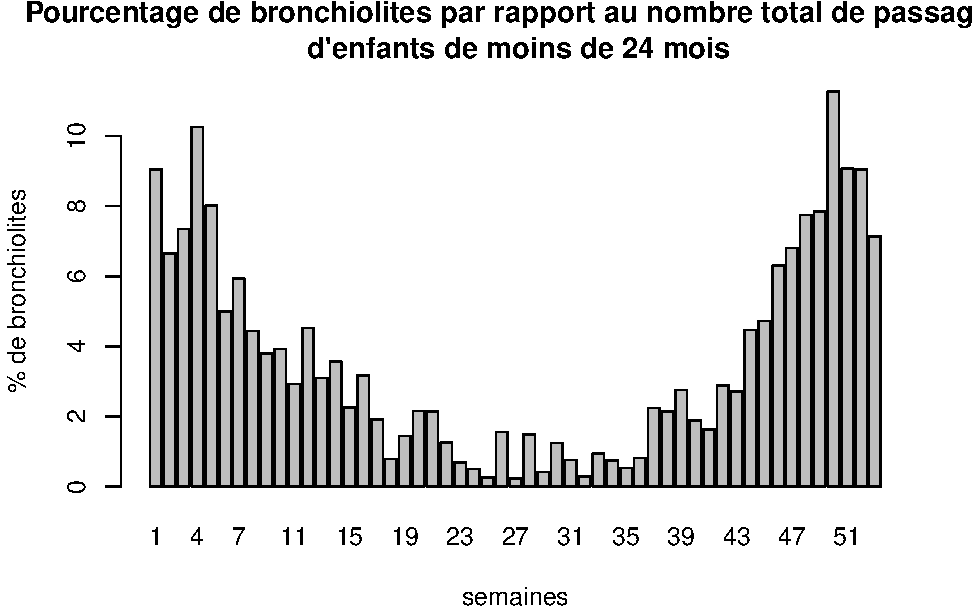
\includegraphics{dp_files/figure-latex/bronchiolites-4.pdf}
\end{figure}

\begin{Shaded}
\begin{Highlighting}[]
\CommentTok{# sous forme de courbe type InVS}
\KeywordTok{plot}\NormalTok{(a, }\DataTypeTok{type=}\StringTok{"l"}\NormalTok{, }\DataTypeTok{xlab =} \StringTok{"semaines"}\NormalTok{, }\DataTypeTok{ylab =} \StringTok{"% de bronchiolites"}\NormalTok{, }\DataTypeTok{main =} \StringTok{"Proportion de bronchiolites parmi le total de passages}\CharTok{\textbackslash{}n}\StringTok{ chez les enfants de moins de 24 mois"}\NormalTok{)}
\end{Highlighting}
\end{Shaded}

\begin{figure}[htbp]
\centering
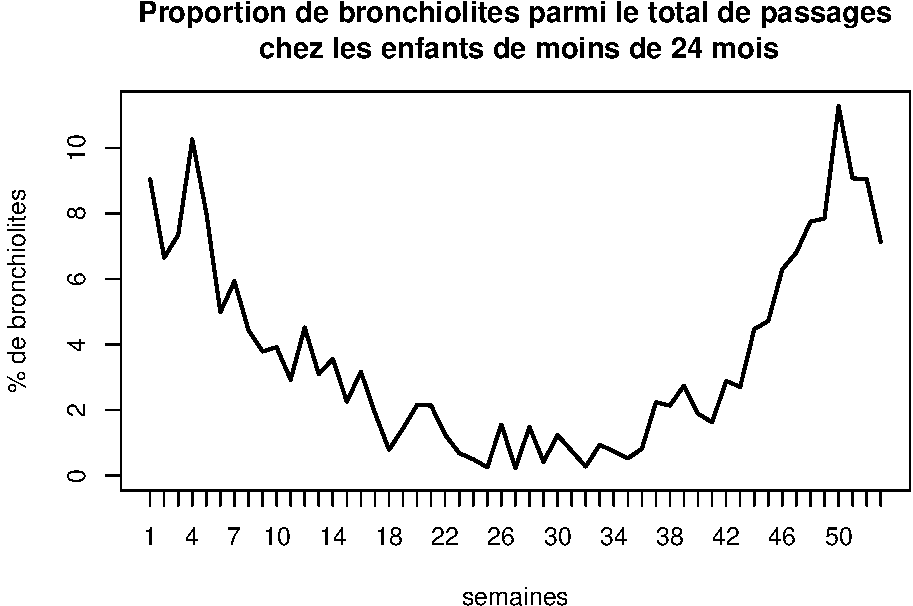
\includegraphics{dp_files/figure-latex/bronchiolites-5.pdf}
\end{figure}

\section{Syndrome grippal}\label{syndrome-grippal}

\textbf{ATENTION}: les gaphiques de ce paragraphe ne sont exact que
\textbf{dpr} ne concerne que 2014. La transformation en mois supprime la
notion d'année =\textgreater{} si plusieurs années, la transformation en
mois entraïne la somme des valeurs dumois: par ex. mois 1 correspond à
la somme janvier 2014 et janvier 2015.

\begin{figure}[htbp]
\centering
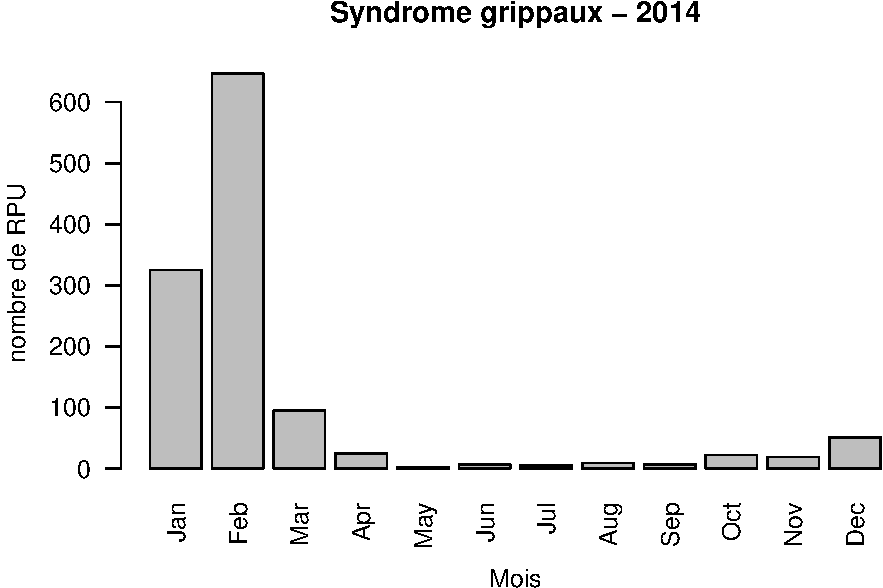
\includegraphics{dp_files/figure-latex/grippe-1.pdf}
\end{figure}

\subsection{Comparaison 2014 - 2015}\label{comparaison-2014---2015}

Utilise 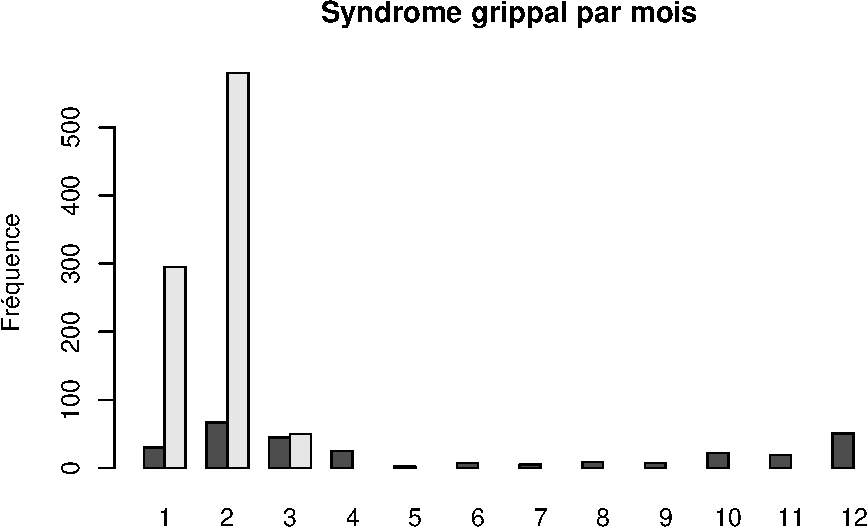
\includegraphics{dp_files/figure-latex/grippe2-1.pdf}
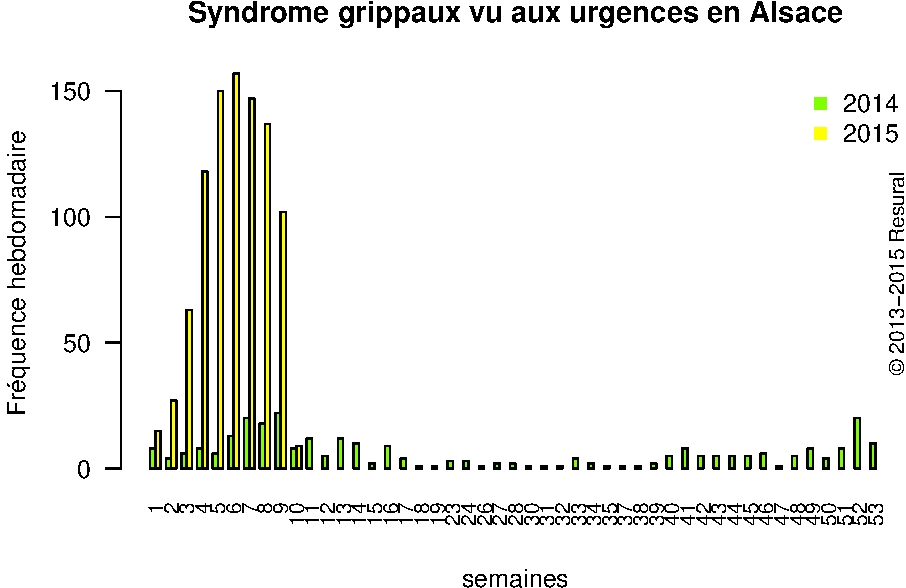
\includegraphics{dp_files/figure-latex/grippe2-2.pdf}
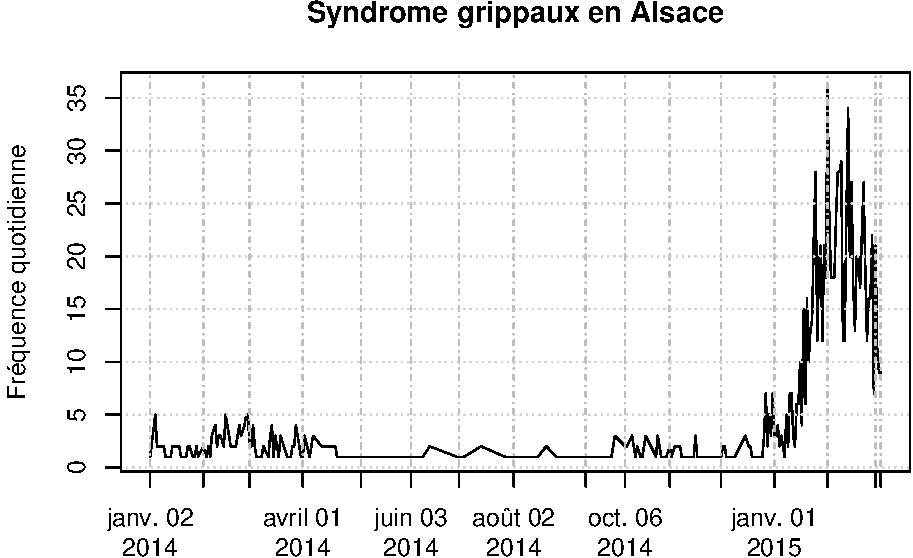
\includegraphics{dp_files/figure-latex/grippe2-3.pdf}
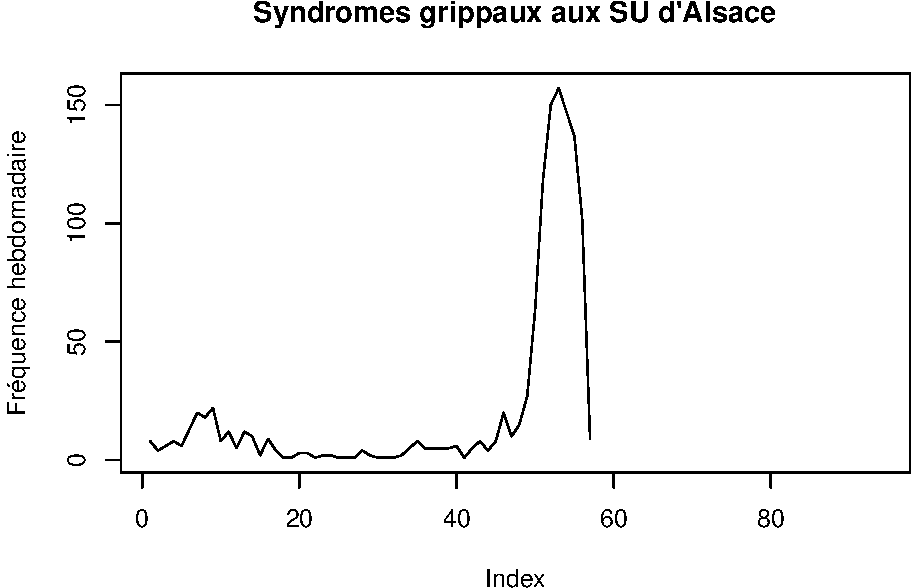
\includegraphics{dp_files/figure-latex/grippe2-4.pdf}
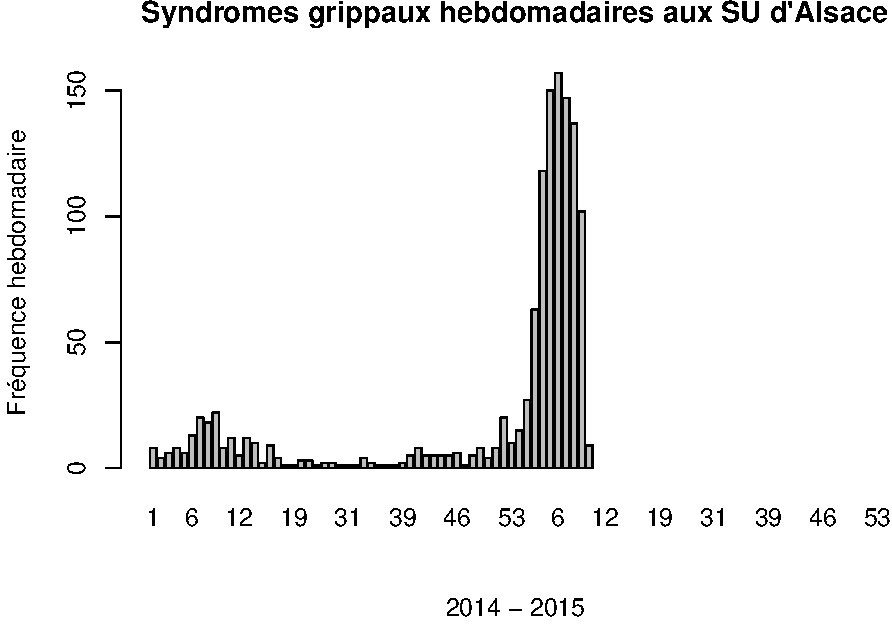
\includegraphics{dp_files/figure-latex/grippe2-5.pdf}

\end{document}
